\section{Evaluation der Implementation mit echten Logdateien}
In diesem Abschnitt haben wir unsere Implementierung für die Analyse von \gls{ssh}-Logdateien der Hochschule verwendet. Um die Dateien zu extrahieren, hat unsere Promtail-Instanz die folgenden Konfigurationen verwendet:

% {\setstretch{1.0}
% \begin{Verbatim}[frame=single,fontsize=\small]
% scrape_configs:
% - job_name: sshlogs
%   decompression:
%     enabled: true
%     initial_sleep: 15s
%     format: gz
%   static_configs:
%   - targets:
%       - localhost
%     labels:
%       job: sshlogs
%       instance: Opfersystem1
%       __path__: /var/log/**.gz
% \end{Verbatim}
% }

\begin{table}[H]
    \setstretch{1}
    \begin{tabularx}{\textwidth}{|m{5.5cm}|X|}
    \hline
    \multicolumn{1}{|c|}{\textbf{Konfigurationsfeld}} & \multicolumn{1}{|c|}{\textbf{Beschreibung}} \\
    \hline
    scrape\_configs & Steht für die Funktionalität von Promtail, automatisch nach Logdateien zu suchen. \\
    \hline
    decompression \newline
    \hphantom{12}enabled: true \newline
    \hphantom{12}initial\_sleep: 10s \newline
    \hphantom{12}format: gz & Promtail kann verschiedene Komprimierungsformate verarbeiten, darunter auch .gz, welches wir in unserer Arbeit verwenden. Das Feld \textit{initial\_sleep} beschreibt das Intervall, bevor die Dekomprimierung beginnt. Dieses Feld kann nützlich sein, wenn komprimierte Dateien vorhanden sind, deren Komprimierungsvorgang jedoch noch nicht abgeschlossen ist. Das Feld \textit{format} gibt das Komprimierungsformat an \citep{Grafana_Promtail}.  \\
    \hline
    static\_configs: \newline
    \hphantom{1}- targets: \newline
    \hphantom{123}- localhost \newline
    \hphantom{1}labels: \newline
    \hphantom{123}job: sshlogs \newline
    \hphantom{123}\_\_path\_\_: /var/log/**.gz & Das Feld \textit{targets} bezieht sich auf die Kommunikation mit der Loki-Instanz. Das Feld \textit{labels} zeigt an, unter welcher Bezeichnung der Inhalt dieser Datei in Loki aufgerufen werden kann. \textit{\_\_path\_\_} gibt den Pfad zur Datei im System an.\\
    \hline
    \end{tabularx}
    \caption[Konfigurationsausschnitt von Promtail]
    {Konfigurationsausschnitt von Promtail}
    \label{tab:KonfigPromtail}
\end{table}

% \begin{table}[H]
%   \setstretch{1}
%   \begin{tabularx}{\textwidth}{|m{5.5cm}|X|}
%   \hline
%   \multicolumn{1}{|c|}{\textbf{Konfigurationsfeld}} & \multicolumn{1}{|c|}{\textbf{Beschreibung}} \\
%   \hline
%   static\_configs: \newline
%   \hphantom{1}- targets: \newline
%   \hphantom{123}- localhost \newline
%   \hphantom{1}labels: \newline
%   \hphantom{123}job: sshlogs \newline
%   \hphantom{123}\_\_path\_\_: /var/log/**.gz & \quotes{targets} bezieht sich auf die Kommunikation mit dem Loki-Instanz. \quotes{labels} zeigt, mit welcher Identifizierung den Inhalt dieser Datei im Loki aufgerufen werden kann. \quotes{\_\_path\_\_} gibt an, wo sich die Datei im System befinden\\
%   \hline
%   %sample\_rate: 0.1 & , which means that Promtail will sample 10% of the series during scraping. \\
%   %\hline
%   \end{tabularx}
%   \caption[Konfigurationsausschnitt von Promtail]
%   {Konfigurationsausschnitt von Promtail}
%   \label{tab:KonfigPromtail}
% \end{table}

Promtail sucht automatisch und in vordefinierten Zeitabständen nach Logdateien, die in der Konfigurationsdatei eingetragen wurden. In Tabelle \ref{tab:KonfigPromtail} finden Sie eine Erklärung jedes Elements dieser Konfiguration.

\quotes{Labels} spielen eine wesentliche Rolle in der Leistung von Loki, da dieses Tool mit weniger Indizierung als andere Tools wie Elastic Stack arbeitet. Laut \cite{Grafana_labels} wird empfohlen, so wenige \quotes{labels} wie möglich zu verwenden und die Extraktion von Inhalten stattdessen mit Hilfe der Abfragesprache durchzuführen, um eine Eskalation des Speicherbedarfs zu vermeiden. Abbildung \ref{fig:Eskalation_Labels} zeigt den Effekt von mehreren \quotes{labels} auf die Anwendung:

\begin{figure}[H]
  \centering
  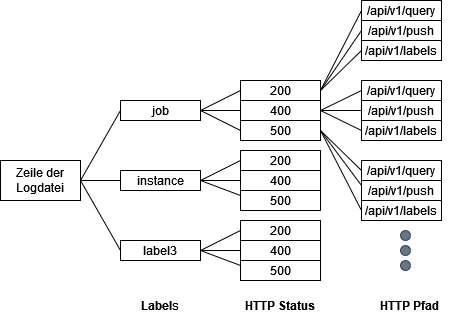
\includegraphics[width=0.7\textwidth]{assets/labelstream.png}
  \caption[Eskalation bei Verwendung von \quotes{labels}]
  {Eskalation bei Verwendung von \quotes{labels} laut \cite{Grafana_labels}}
  \label{fig:Eskalation_Labels}
  \centering
\end{figure}

Auf Abbildung \ref{fig:Eskalation_Labels} haben wir vier Ebenen. Die erste Ebene ist die Zeile der Logdatei (1), die zweite Ebene sind die vom Benutzer definierten \quotes{labels} (2), und die dritte und vierte Ebene beziehen sich auf die Antwort (3) und die verwendete HTTP-Anfrage (4), um nach Inhalten zu suchen, sie hinzuzufügen und zu indizieren. Aus einer Zeile der Logdatei haben wir drei \quotes{labels} definiert (3x), die wiederum drei potenzielle Zustände haben (3x3x), und aus diesen drei Zuständen haben wir drei mögliche HTTP-Pfade (3x3x3). Das ergibt insgesamt 27 Streams, um die Zeile zu lesen, zu indizieren und zu speichern. Dies kann laut \cite{Grafana_labels} zu einer Beeinträchtigung der Leistung führen.

Unsere Logdateien haben eine Größe von ungefähr vier Megabyte, was im Vergleich zu produktiven Umgebungen, in denen Logdateien den Terabyte-Bereich erreichen können, gering ist. Trotz dieser Größe war unsere Synchronisierung nicht immer so präzise wie erwartet. Einige Abfragen, die bei der Implementierung mit 40 KB Logdateien einwandfrei funktionierten, führten hier zu folgender Fehlermeldung:

{\setstretch{1.0}
\begin{Verbatim}[fontsize=\small, frame=single]
maximum of series (500) reached for a single query  
\end{Verbatim}
}

Die offizielle Dokumentation und die verschiedenen Foren konnten uns keine endgültige Lösung mit der neuesten Version von Loki (2.8.2) bieten. Die verschiedenen Kombinationen in der Konfigurationsdatei von Loki führten immer zum selben Ergebnis. Zum Zeitpunkt unserer Arbeit (19.5.2022) haben wir versucht, über das GitHub-Forum Kontakt mit dem Grafana Loki-Team aufzunehmen, um mögliche Lösungsansätze zu finden.

Mit der Verwendung der Version 2.4.1 konnten wir die oben genannte Situation teilweise lösen. Unsere Abfragen wurden erfolgreich gesendet und die Diagramme wurden generiert. Der folgende Ausschnitt der Loki-Konfiguration in Tabelle \ref{tab:KonfigLoki} half dabei, die Leistungsparameter der Anwendung zu definieren:

% {\setstretch{1.0}
% \begin{Verbatim}[fontsize=\small, commandchars=\\\{\},frame=single]
% \textbf{\textcolor{blue}{limits_config:}}
%   reject_old_samples: true
%   reject_old_samples_max_age: 168h
%   ingestion_rate_mb: 1024
%   ingestion_burst_size_mb: 1024
%   ingestion_rate_strategy: local
%   per_stream_rate_limit: 12MB
%   max_query_series: 100000
%   max_query_parallelism: 32
%   split_queries_by_interval: 24h
%   max_query_length: 0h

% \textbf{\textcolor{blue}{querier:}}
%   max_concurrent: 2048

% \textbf{\textcolor{blue}{frontend:}}
%   max_outstanding_per_tenant: 4096
%   compress_responses: true
%   scheduler_worker_concurrency: 20


% \textbf{\textcolor{blue}{chunk_store_config:}}
%   max_look_back_period: 0s

% \textbf{\textcolor{blue}{table_manager:}}
%   retention_deletes_enabled: false
%   retention_period: 360s
% \end{Verbatim}
% }

\begin{table}[H]
  \setstretch{1}
  \begin{tabularx}{\textwidth}{|p{7cm}|X|}
  \hline
  \multicolumn{1}{|c|}{\textbf{Konfigurationsfeld}} & \multicolumn{1}{|c|}{\textbf{Beschreibung}} \\ \hline
  \textbf{limits\_config:} & Festlegung der Aufnahmerate; \\
  \hphantom{10}reject\_old\_samples: true & Aufnahme von alten Proben;\\ 
  \hphantom{10}reject\_old\_samples\_max\_age: 168h & Aufnahme von alten Proben, wenn sie älter als dieser Wert sind;\\
  \hphantom{10}ingestion\_rate\_mb: 1024 & Aufnahmerate in Megabyte pro Sekunde;\\ 
  \hphantom{10}ingestion\_burst\_size\_mb: 1024 & Aufnahmerate bei einer einzigen Weiterleitung in Megabyte; \\ 
  \hphantom{10}ingestion\_rate\_strategy: local &  Aufnahmerate wird entweder \quotes{local} definiert oder auf \quotes{global} aufgeteilt;  \\ 
  \hphantom{10}per\_stream\_rate\_limit: 12MB & Aufnahmerate in Byte pro Sekunde und pro Stream; \\ 
  \hphantom{10}max\_query\_series: 100000 & Maximale Anzahl von einzelnen Serien pro Abfrage; \\ 
  \hphantom{10}max\_query\_parallelism: 32 & Maximale Anzahl von parallelen Abfragen; \\ 
  \hphantom{10}split\_queries\_by\_interval: 24h & Trennung von Abfragen nach einem definierten Intervall;;\\ 
  \hphantom{10}max\_query\_length: 0h & Grenze für die Ausführungszeit. Dadurch wird eine Überlastung der Rechenkapazität vermieden; \\ 
  \bottomrule
  \end{tabularx}
\end{table}

\begin{table}[H]
  \setstretch{1}
  \begin{tabularx}{\textwidth}{|b{7cm}|X|}
  \hline
  \multicolumn{1}{|c|}{\textbf{Konfigurationsfeld}} & \multicolumn{1}{|c|}{\textbf{Beschreibung}} \\ \hline
  \textbf{querier:} & Einstellung für die Abfrage; \\ 
  \hphantom{10}max\_concurrent: 2048 & Anzahl der gleichzeitigen Abfragen;\\ \hline
  \textbf{frontend:} & Einstellung für die Abfrage im \gls{frontend};\\
  \hphantom{10}compress\_responses: true &Komprimierung der \gls{http}-Antworten;\\
  \hphantom{10}scheduler\_worker\_concurrency: 20 &  Anzahl der gleichzeitigen Abfragen, die verarbeitet werden; \\  \hline
  \textbf{table\_manager:} & Verwaltung der Vorratsdatenspeicherung;\\ 
  \hphantom{10}retention\_deletes\_enabled: false & Löschen von Tabellen in der Datenbank;\\ 
  \hphantom{10}retention\_period 360s & Tabellen werden gelöscht, wenn sie älter als dieser Wert sind;\\ \hline
  \end{tabularx}
  \caption[Konfigurationsausschnitt für Loki]
  {Konfigurationsausschnitt für Loki}
  \label{tab:KonfigLoki}
\end{table}

Trotz dieser Situation waren wir in der Lage, eine allgemeine Warnmeldung für eine hohe Anzahl von fehlgeschlagenen Anmeldeversuchen zu implementieren. Diese Warnmeldung ermöglicht es uns, potenzielle Sicherheitsbedrohungen zu erkennen und angemessen darauf zu reagieren.



% \newpage
% \newgeometry{right=30mm, left=30mm} 
% \thispagestyle{lscape}
% \begin{landscape}
%    Nach manuellen Aktualiserung sah unsere Graphik so aus:
%     \begin{figure}[H]
%        % \centering
%         \centerline{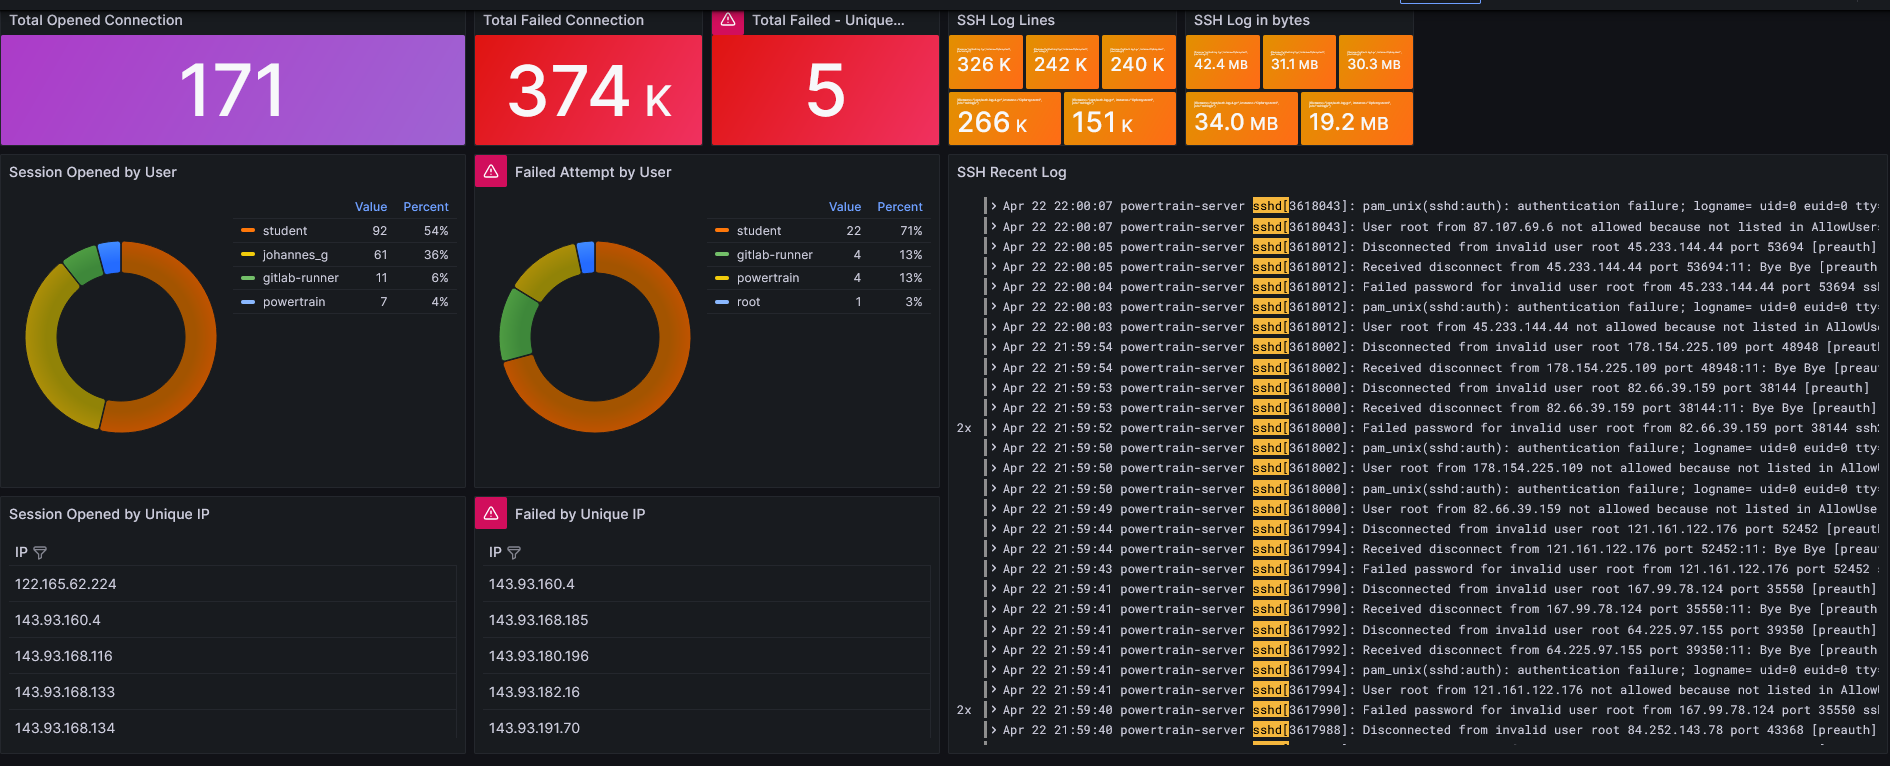
\includegraphics[width=1.8\textwidth]{assets/unserssh}}
%         %\includegraphics[width=1.2\textwidth]{assets/5.4.2_1_Abb.jpeg}
%         \caption[Ausgabe in Grafana von unseren \gls{ssh} Logdateien]
%         {Ausgabe in Grafana von unseren \gls{ssh} Logdateien}
%         \label{fig:Unserssh}
%         \centering
%     \end{figure} 
% \end{landscape}
% \restoregeometry


